\chapter{NES FPGA alapú újra gondolása}

A diplomaterv projektem egyik fő célja, egy hardveres emulátort készítsek a Nintendo Entertainment System játékkonzolhoz. Alapvetően emulátort lehet készíteni szoftveres illetve hardveres módon. A szoftveres emulátorok alapja az eredeti hardver szimulálása egy szoftver segítségével a lehető pontosabb módon (ez nem minden esetben sikerül). Hardveres emulálásnál általában egy FPGA chipet használnak és ezen definiálják az eredeti hardveres működéseket. Az általunk választott megvalósítás sokkal idő igényesebb, viszont ennek segítségével képesek vagyunk az eredeti eszköz legpontosabb emulálására. Illetve egy erősebb FPGA segítségével modernizálhatunk egy régebbi konzolt is, persze bármilyen hardveres módosítás esetén (amely eltér az eredeti eszköztől), át kell gondolnunk, hogy a megváltozott körülmények között is minden működni fog-e az eredeti hardverben. 

Ebben a fejezetben azt fogom bemutatni, hogy milyen hardveres változtatásokat/fejlesztéseket eszközöltem, az eredeti NES-hez képest, hogy egy friss, modernebb megjelenést adjak az eredeti konzolnak.

\section{Képalkotás}

Már az előző \ref{subsec:PPU-CRT} fejezetben olvashattuk, hogy a NES egy kompozit jelet állított elő CRT televíziók számára. Ez talán a játé konzol legelavultabb része, hiszen napjainkban már ezt a televízió típust nem is lehet beszerezni. Ezeket teljes mértékben leváltották a VGA alapú (DVI, HDMI, DisplayPort csatlakozóval ellátott) különböző méretű és felbontású lapos TV-k. Ezeknek a megvalósításoknak rengeteg előnye van az analóg megjelenítéssel szemben. Az egyik legjelentősebb, hogy ezen keresztül képesek vagyunk torzításmentes átvitelre.

A NES eredeti felbontása 256 x 240 pixel és 60 Hz (NTSC). Ez a  méret sajnos nem felel meg a modern VGA szabványoknak, úgy hogy ezen a téren módosítanunk kell a PPU képgenerálásán. A módosítások során a VGA adatok generálását helyeztem elő térbe. A legkisebb VGA kép méret amivel érdemes dolgozni és a modern TV-k és monitorok támogatnak az a 640 x 480 pixel és 60 Hz, szerencsénkre ebbe a méretbe pontosan elfér a kétszeres NES kép méret. Ebből eredeztetve, ha egy pixel-t 2 x 2 pixel-el reprezentálunk, akkor 512 x 480 pixel méretű képet kapunk ennél bonyolultabb megoldás is létezik (bilineáris interpoláció), de ez a legegyszerűbb ezért kezdetben ezt implementálom. Ez a változtatás lehetővé teszi, hogy NES nyomtatott huzalozott kártyáján modern HDMI csatlakozót helyezzek el. 

Illetve ebből a módosításból következőleg a rendszerünk működési frekvenciája is megváltozik, a VGA jelünk pixel óra jele 25 Mhz lesz, az RGB adatok pedig 250 Mhz-el lesznek továbbítva a TV vagy monitor felé. Ez azt jelenti, hogy a PPU-nk működési órajelét is meg kell változtatni (eredetileg körülbelül 5.37MHz NTSC modellben). A NES nyomtatott huzalozott kártyáján ezért egy magasabb órajelforrást kell elhelyezni. Az órajel pontos beállítására pedig az FPGA chip DCM (Digital Clock Manager) és PLL (Phase Locked Loop) funkcióit használhatjuk.  

\section{Audio}
%todo fűzd össze a audio bemutatásával
Az Audio Process Unit (APU), egy öt külön álló hangsávot kezelő komponens, mely a NES eredeti hangját, nem lineáris keverés segítségével állította elő ezekből a csatornákból. Ezt a jelet a hardveres emulálás során mi egy digitális jelként állítjuk elő az FPGA-val. Ahhoz, hogy eredeti eszköz hangját élvezni tudjuk ezt először egy DAC segítségével analóg jellé kell konvertálnunk, végül pedig egy megfelelő erősítőn át egy Jack csatlakozóra kivezetnünk. Az erősítő típusa attól függ, hogy fülhallgatón vagy pedig hangszórón szeretnénk, hogy ezek az ikonikus dallamok megszólaljanak. Egy jó kompromisszumos megoldás a kártyát fülhallgató erősítővel ellátni mivel hangszórókból léteznek olyan modellek (belső erősítővel rendelkezők), amelyek ezzel az gyengébb erősítővel is működnek (így mind a két opció fennáll a konzol használatra). Az eredeti konzol mono hangzással rendelkezett viszont mi ezt jelet a DAC működése miatt, mind a két fülre kivezethetjük, ezzel sztereó hangzást imitálva (ettől még természetesen ez nem lesz valódi sztereó jel).   

Mivel a NES nyomtatott huzalozott kártyáján már a képalkotás miatt elhelyezek egy HDMI csatlakozót, ezért egy kisebb I2C szint illesztő komponens segítségével a HDMI hang csatornái is beköthetők. Így lehetővé téve, hogy egy esetleges későbbi fejlesztés során a TV/monitor beépített hangszóróján szólaljon meg játékkonzolunk. 

\section{Játékok tárolása}
\label{sec:Game-store}
%todo fűzd össze a kazetták bemutatásával
A NES játékok programkódja és Pattern tábla adatai az esetek többségében a játék kazetta saját program és karakter ROM-jában helyezkedtek el. Ez a megoldás rengeteg extra területet emésztene fel a nyomtatott huzalozott kártyán (a kazetta befogadó egységet rá kéne tervezni az eszközre), illetve az összes teszt játéknak fizikailag a birtokomba kell lennie ehhez (és egyéb hardveres teszteket nehezen lehetne megvalósítani). 

Ennek következtében egy új megoldást kellet kitalálni arra, hogy az emulált NES hardvert megfelelő módon ellássam játékokkal. Az egyik kézen fekvő megoldás, hogy a hordozó kártyára el lehet helyezni egy statikus RAM modult amelynek elég nagynak kell lennie ahhoz, hogy a játék kártyák karakter és program ROM-ját egyszerre tartalmazza. A legnagyobb NES játék 768 KB memória területtel rendelkezett és ez a Kirby's Adventure volt, ehhez képest az összes többi játék 512 KB-os vagy ennél kisebb volt. A NES hardver indítás előtt ezt a SRAM-ot fel kell töltenünk a játékkal, majd a hardver indítását követően a PPU és CPU innen fog dolgozni.

Annak érdekében, hogy több játékot is képesek legyünk tárolni érdemes egy nagyobb méretű háttértárat is tervezni az eszközre, amely a játékokat fogja tartalmazni, erre ideális lehet egy SD kártya. A projekt kezdeti szakaszában ezt még nem használom, viszont az esetleges jövőbeli fejlesztések miatt érdemes, már most a kártyára tervezni egy ilyen olvasót.

A NES hardver játék megjelenítéshez szükséges belső memória területeit, pedig az FPGA-ba kialakítható Block/LUT ram-ba helyezhetjük helyezhetjük el (Név táblák, OAM, másodlagos OAM).

\section{Kompakt hordozható méret}
\label{sec:Size}

A NES újra tervezésének egyik fő aspektusa a méret csökkentése. Az eredeti konzol 256 mm hosszú, 203.2 mm széles és 88.9 mm vastag volt. Ezt a modern nyomtatott áramkörök tervezésével, és a komponensek kis méretével sokkal kisebb területre csökkenthető. Ezzel kompakt hordozható kialakítást kölcsönözve a játék konzolnak.

%todo fekete fehét kép
\begin{figure}[H]
	\centering
	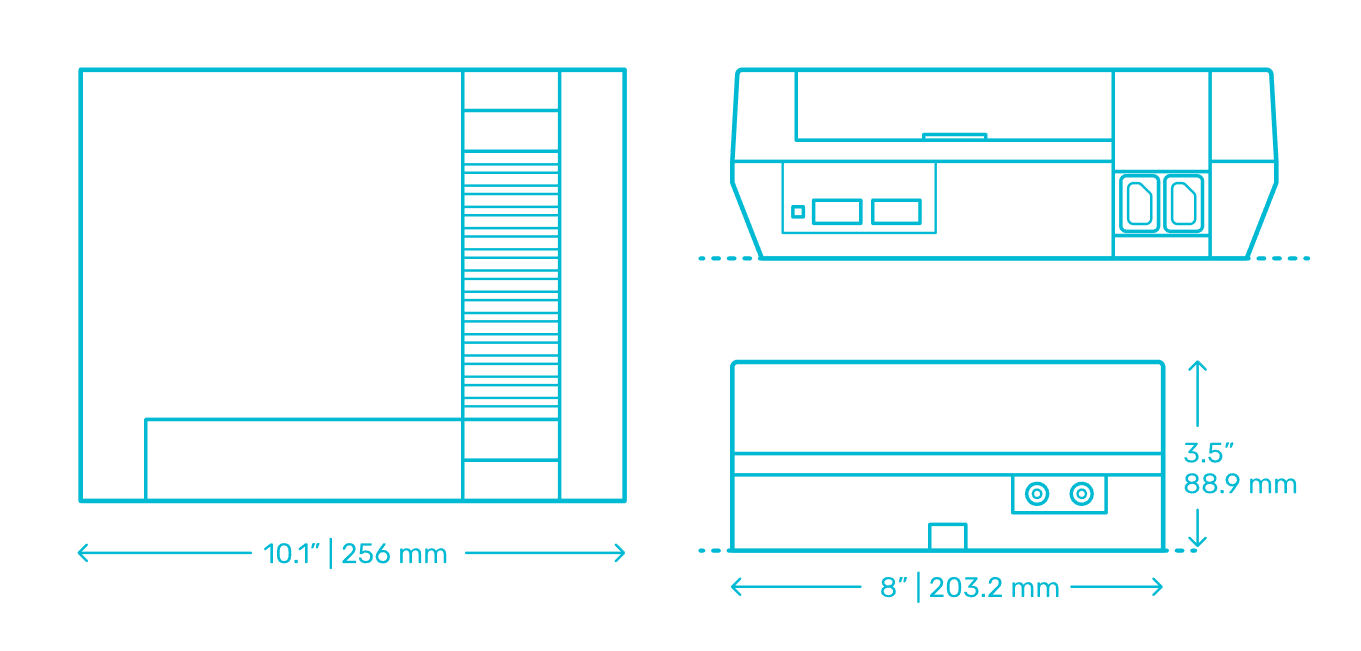
\includegraphics[width=150mm, keepaspectratio]{figures/NES-size}
	\caption{A NES játék konzol dimenziói}
	\label{fig:NES-size}
\end{figure}

A kompakt méret mellet szerettem volna megőrizni az eszköz nosztalgia faktorát, ezért a kártyámon elhelyeztem két eredeti NES játék kontroller csatlakozót (kooperatív játékok miatt). Ez természetesen az eredeti hardver kontrollereivel kompatibilis.


